\section{Theoretical Analysis}
\label{sec:analysis}


Similar to what was done on the simulation analysis, we began by determining the voltages in all the nodes, and currents in all the branches, for $t<0$. That amounts to $v_s=V_s$, and therefore, to there being no changes in the currents in all the branches for that time interval, and thus, the capacitor behaving as a open circuit. To do this analysis, we used the nodal method to obtain all the equations necessary, and then used Octave to get the numerical results. Octave was also used during the rest of this Theoretical Analysis.
 

%matriz
\begin{equation}
\begin{pmatrix}
1 & 0 & 0 & 0 & 0 & 0 & 0\\
\frac{-1}{R_1} & \frac{1}{R_1} + \frac{1}{R_2} + \frac{1}{R_3} & \frac{-1}{R2} & \frac{-1}{R_3} & 0 & 0 & 0\\
0 & \frac{1}{R_2} + K_b & \frac{-1}{R_2} & -K_b & 0 & 0 & 0\\
\frac{-1}{R1} & \frac{1}{R_1} & 0 & \frac{1}{R_4} & 0 & \frac{1}{R_6} & 0\\
0 & 0 & 0 & 1 & 0 & \frac{K_d}{R_6} & -1\\
0 & K_b & 0 & \frac{-1}{R_5} - K_b & \frac{1}{R_5} & 0 & 0\\
0 & 0 & 0 & 0 & 0 & \frac{-1}{R_6} - \frac{1}{R_7} & \frac{1}{R_7}\\


\end{pmatrix}
\begin{pmatrix}
V_1\\
V_2\\
V_3\\
V_5\\
V_6\\
V_7\\
V_8\\
\end{pmatrix}
=
\begin{pmatrix}
V_s\\
0\\
0\\
0\\
0\\
0\\
0\\
\end{pmatrix}
\label{eq:MatrixKCL}
\end{equation}

%resultados

\begin{table}[h!]
  \centering
  \begin{tabular}{|l|r|}
    \hline    
    {\bf $V_i$} & {\bf Value [V]} \\ \hline
    $V_1$ & 5.134559 V\\ 
$V_2$ & 4.871563 V\\ 
$V_3$ & 4.321260 V\\ 
$V_4$ & 4.908647 V\\ 
$V_5$ & 5.722227 V\\ 
$V_6$ & -1.876518 V\\ 
$V_7$ & -2.800822 V\\ 

    \hline
  \end{tabular}
  \caption{Nodal analysis results for $t < 0$ s}
  \label{tab:Nodal}
\end{table}


We then determined the equivalent resistance $R_{eq}$ as seen from the capacitor terminals. This is achieved by making $V_s=0$ and replacing the capacitor by a voltage source $V_x=V(6)-V(8)$, where $V(6)$ and $V(8)$ are the previously obtained voltages on node 6 and node 8, respectively. Then, we ran nodal analysis to determine the current $I_x$ supplied by the voltage source $V_x$. This way, it was possible to compute $R_eq= \frac{V_x}{I_x}$. (explicar porque é que é possível fazer isso) We obtained the following results:

%equações etc%

\begin{equation}
\begin{pmatrix}

\frac{1}{R_1} + \frac{1}{R_2} + \frac{1}{R_3} & \frac{-1}{R2} & \frac{-1}{R_3} & 0 & 0 & 0 & 0\\
\frac{1}{R_2} + K_b & \frac{-1}{R_2} & -K_b & 0 & 0 & 0 & 0\\
\frac{1}{R_1} & 0 & \frac{1}{R_4} & 0 & \frac{1}{R_6} & 0 & 0\\
0 & 0 & 1 & 0 & \frac{K_d}{R_6} & -1 & 0\\
K_b & 0 & \frac{-1}{R_5} - K_b & \frac{1}{R_5} & 0 & 0 & -1\\
0 & 0 & 0 & 0 & \frac{-1}{R_6} - \frac{1}{R_7} & \frac{1}{R_7} & 0\\
0 & 0 & 0 & 1 & 0 & -1 & 0\\


\end{pmatrix}
\begin{pmatrix}
V_2\\
V_3\\
V_5\\
V_6\\
V_7\\
V_8\\
I_x\\
\end{pmatrix}
=
\begin{pmatrix}
0\\
0\\
0\\
0\\
0\\
0\\
V_x\\
\end{pmatrix}
\label{eq:NodalVs0}
\end{equation}

%tabela
\begin{table}[h!]
  \centering
  \begin{tabular}{|l|r|}
    \hline    
    {\bf Name} & {\bf Value [V or mA or kOhm or ms]} \\ \hline
    $V_2$ & 0.000000 V\\ 
$V_3$ & 0.000000 V\\ 
$V_5$ & 0.000000 V\\ 
$V_6$ & 8.523049 V\\ 
$V_7$ & -0.000000 V\\ 
$V_8$ & -0.000000 V\\ 
$I_x$ & 2.833761 mA\\ 
$R_{eq}$ & 3.007681 mA\\ 
$\tau$ & 3.115171 ms\\ 

    \hline
  \end{tabular}
  \caption{Nodal analysis resutls for $t < 0$s and $V_s = 0$V }
  \label{tab:Nodal2}
\end{table}


With these results, we determined the equivalent differential equation for $v_{6}$, and solved it using $V_x$ as an initial condition. This way, we obtained the natural solution $v_{6n}(t)$, for the node voltage $v_{6}$, in the interval $[0, 20]$ms. 



%%%%%%%%%%%%%NATURAL
%Sinal resultado
$$8.523048798 e^{- 0.32100971396 t}$$

%plot 
\begin{figure}[h!] \centering
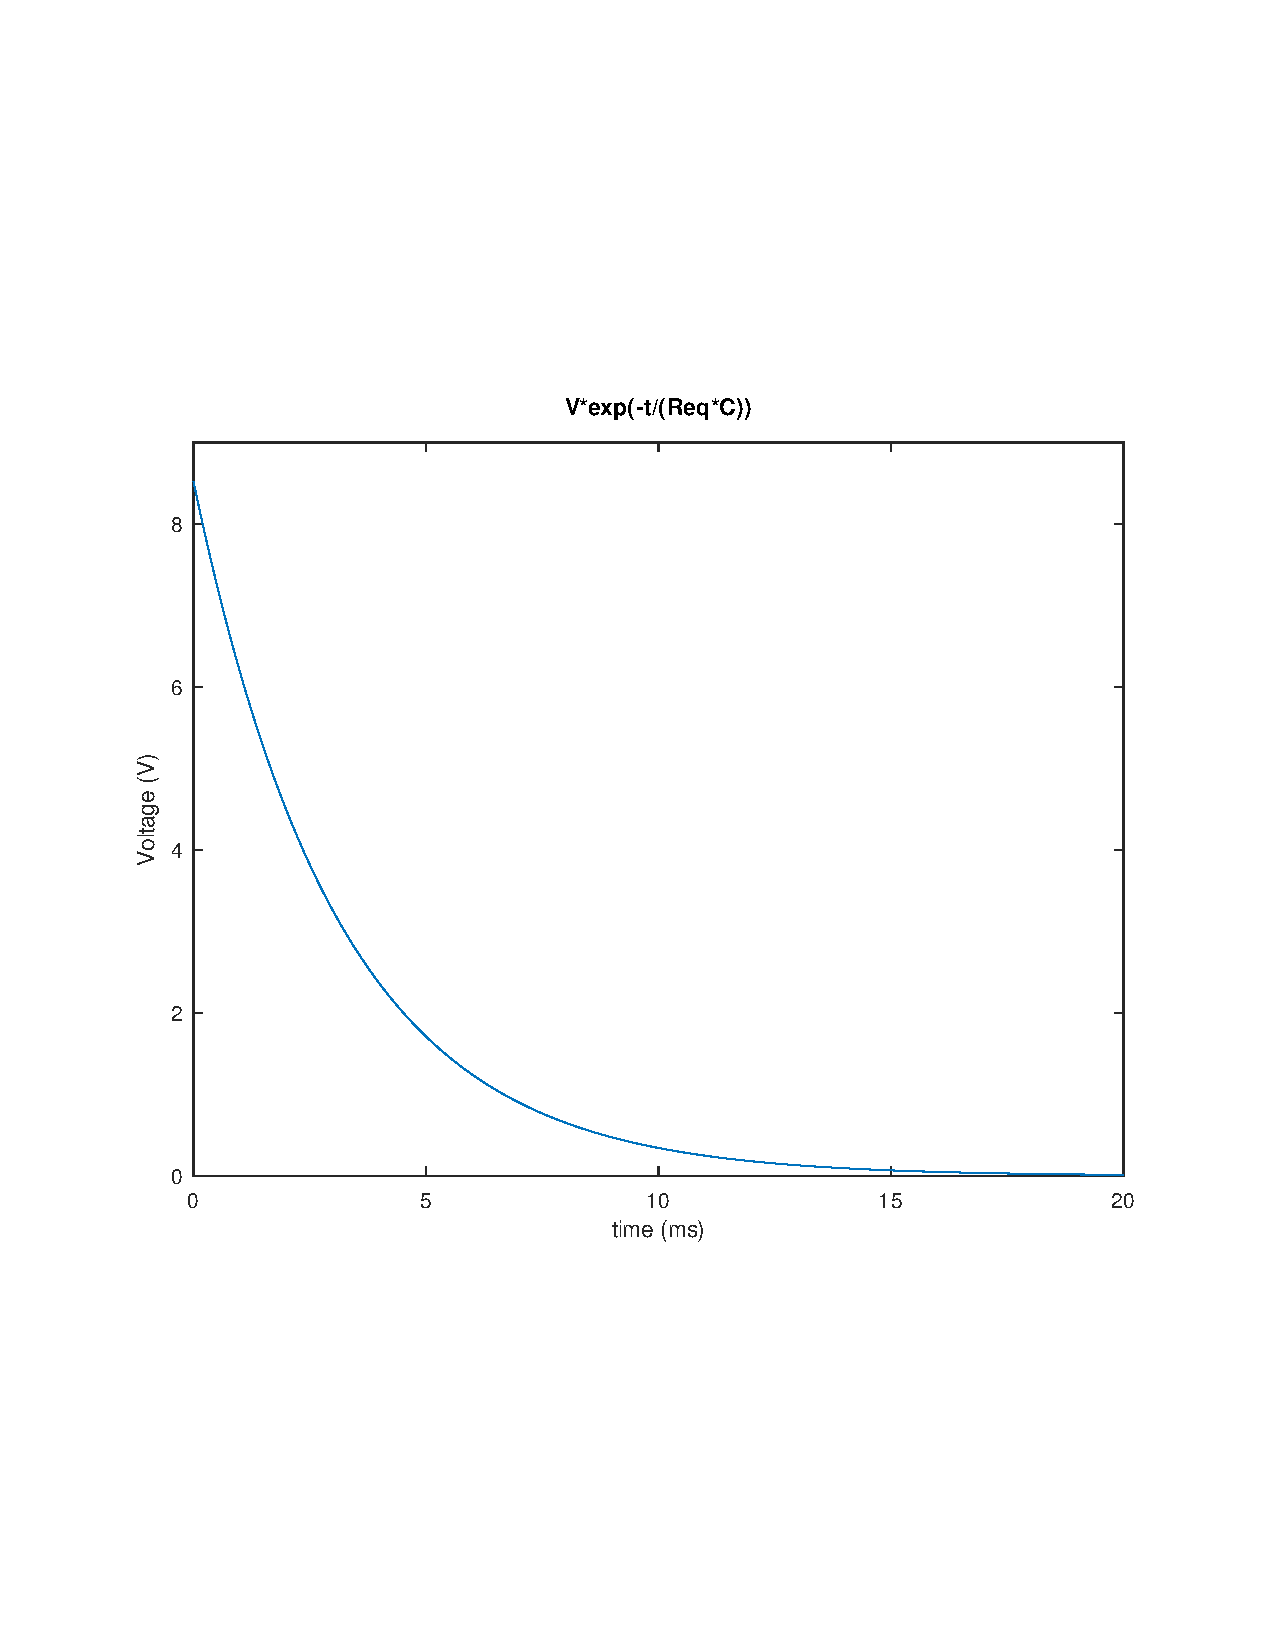
\includegraphics[width=0.6\linewidth]{../mat/natural.pdf}
\caption{Natural solution}
\label{fig:TNatural}
\end{figure}


%%%%%%%%%%%%%%%%%%%%%%%%%%%%%%%%%%%%%%%%%%%%%%%%%FORÇADO 
The next step to obtain the full solution for $v_6(t)$ is to obtain the forced solution $v_{6f}(t)$, in that same time interval. With that objective in mind, we started by replacing the capacitor for its equivalent impedance $Z_c=\frac{1}{j\,\omega \, C}$ That way, we can obtain equations that are similar to (fazer referência às primeiras equações da análise), by again running a nodal analysis of the circuit. By making $V_s=0$, and solving this system of equations, we obtain phasor voltages for all the nodes. In this case, $f=1$ kHz.

%resultados, eqauções, whatever the fuck
%equação matricial 
\begin{equation}
\begin{pmatrix}
1 & 0 & 0 & 0 & 0 & 0 & 0\\
\frac{-1}{R_1} & \frac{1}{R_1} + \frac{1}{R_2} + \frac{1}{R_3} & \frac{-1}{R2} & \frac{-1}{R_3} & 0 & 0 & 0\\
0 & \frac{1}{R_2} + K_b & \frac{-1}{R_2} & -K_b & 0 & 0 & 0\\
\frac{-1}{R1} & \frac{1}{R_1} & 0 & \frac{1}{R_4} & 0 & \frac{1}{R_6} & 0\\
0 & 0 & 0 & 1 & 0 & \frac{K_d}{R_6} & -1\\
0 & K_b & 0 & \frac{-1}{R_5} - K_b & \frac{1}{R_5} + jC\omega & 0 & -jC\omega\\
0 & 0 & 0 & 0 & 0 & \frac{-1}{R_6} - \frac{1}{R_7} & \frac{1}{R_7}\\


\end{pmatrix}
\begin{pmatrix}
\tilde{V_1}\\
\tilde{V_2}\\
\tilde{V_3}\\
\tilde{V_5}\\
\tilde{V_6}\\
\tilde{V_7}\\
\tilde{V_8}\\
\end{pmatrix}
=
\begin{pmatrix}
V_s\\
0\\
0\\
0\\
0\\
0\\
0\\
\end{pmatrix}
\label{eq:MatrixKCL}
\end{equation}

%%PHASOR TABLE
\begin{table}[h!]
  \centering
  \begin{tabular}{|l|r|}
    \hline    
    {\bf Name} & {\bf Value [V]} \\ \hline
    $abs(V_1)$ & 1.000000 V\\ 
$abs(V_2)$ & 0.948779 V\\ 
$abs(V_3)$ & 0.841603 V\\ 
$abs(V_5)$ & 0.956002 V\\ 
$abs(V_6)$ & 0.547734 V\\ 
$abs(V_7)$ & 0.365468 V\\ 
$abs(V_8)$ & 0.545484 V\\ 

    \hline
  \end{tabular}
  \caption{Nodal analysis resutls for $t < 0$s and $V_s = 0$V }
  \label{tab:Nodal2}
\end{table}



To finally obtain the forced solution $v_{6f}(t)$, we converted the phasors to real time solutions of the form $v_{6f}(t) = A\, cos(\omega t+ \, \phi)$: the norm of the phasor corresponding to the amplitude $A$ of the solution and the the argument corresponding to the phase $\phi$. We obtained the following solution for $v_{6f}(t)$ on time interval $[0,20]$ ms:

%equação
$$0.54773358245 \sin{\left(6.2831853071795862319959269370884 t - 2.9865432432 \right)}$$

%plot 
\begin{figure}[h!] \centering
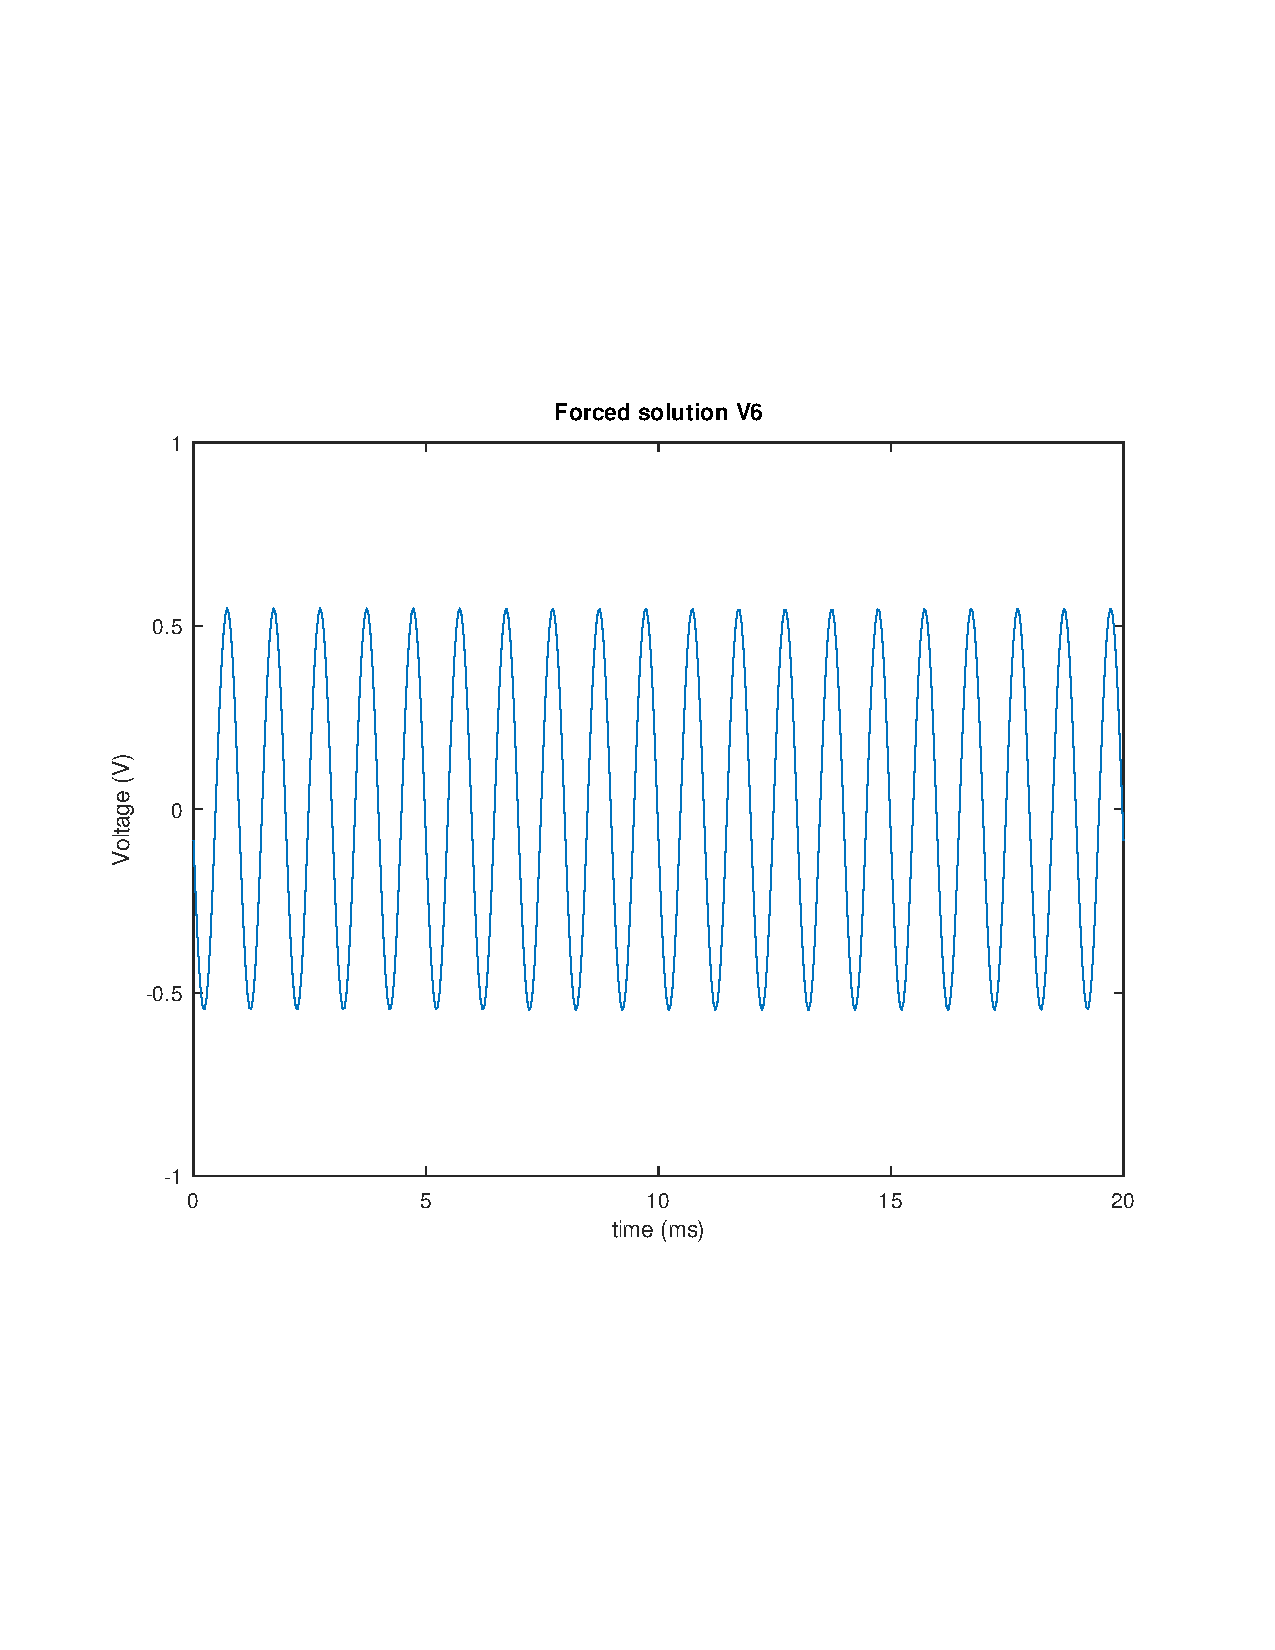
\includegraphics[width=0.6\linewidth]{../mat/forced_1.pdf}
\caption{Forced solution $t > 0$s}
\label{fig:TForcedP}
\end{figure}

%%%%%%%%%%%%%%%%%%%%%%%%%%%%%%%%%%%%%%%%%%%%%%%%%%%%%%TOTAL SOLUTION 	

The total solution $v_6(t)$ is computed by summing the two solutions obtained beforehand, the natural solution $v_{6n}(t)$ and the forced solution $v_{6f}(t)$.
%equação
$$0.54773358245 \sin{\left(6.2831853071795862319959269370884 t - 2.9865432432 \right)} + 8.523048798 e^{- 0.32100971396 t}$$

%plots
\begin{figure}[h!] \centering
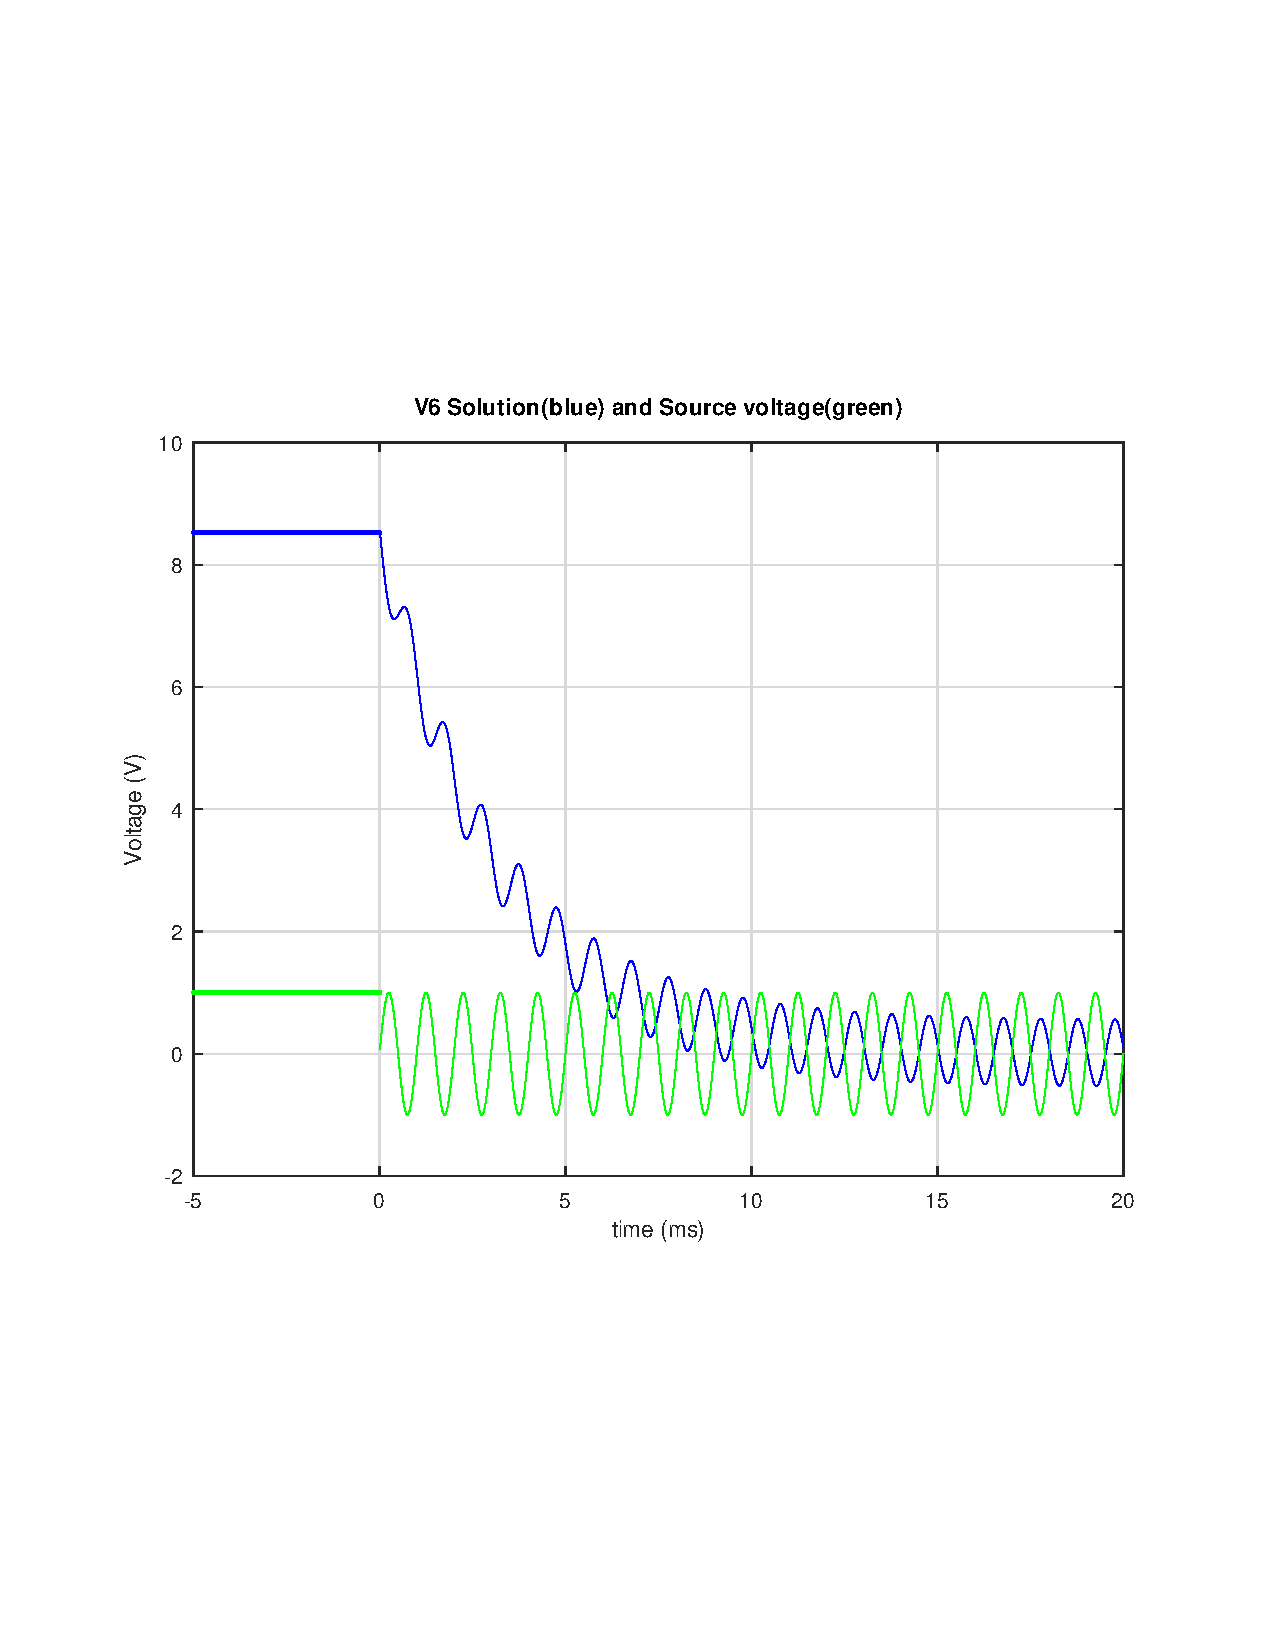
\includegraphics[width=0.6\linewidth]{../mat/fullSolution.pdf}
\caption{Forced solution $t > 0$s}
\label{fig:TForcedP}
\end{figure}


%%%%%%%%%%%%%%%%%%%%%%%%%%%%%%%%%%%%Transfer function 
%figuras bonitas 
We finally explored the frequency responses (transfer function) $v_c(f)= v_6(f)-v_8(f)$ to the frequency $f$ of the voltage source. 
$$\frac{- 2.58398734354048 \cdot 10^{72} i f + 2.69716941607415 \cdot 10^{71}}{4.73705055795528 \cdot 10^{72} i f + 2.4201725243886 \cdot 10^{71}}$$
$$\frac{3.92318858461668 \cdot 10^{56} i f + 4.0173358562871 \cdot 10^{71}}{4.73705055795528 \cdot 10^{72} i f + 2.4201725243886 \cdot 10^{71}}$$

The following plots were obtained:

\begin{figure}[h!] \centering
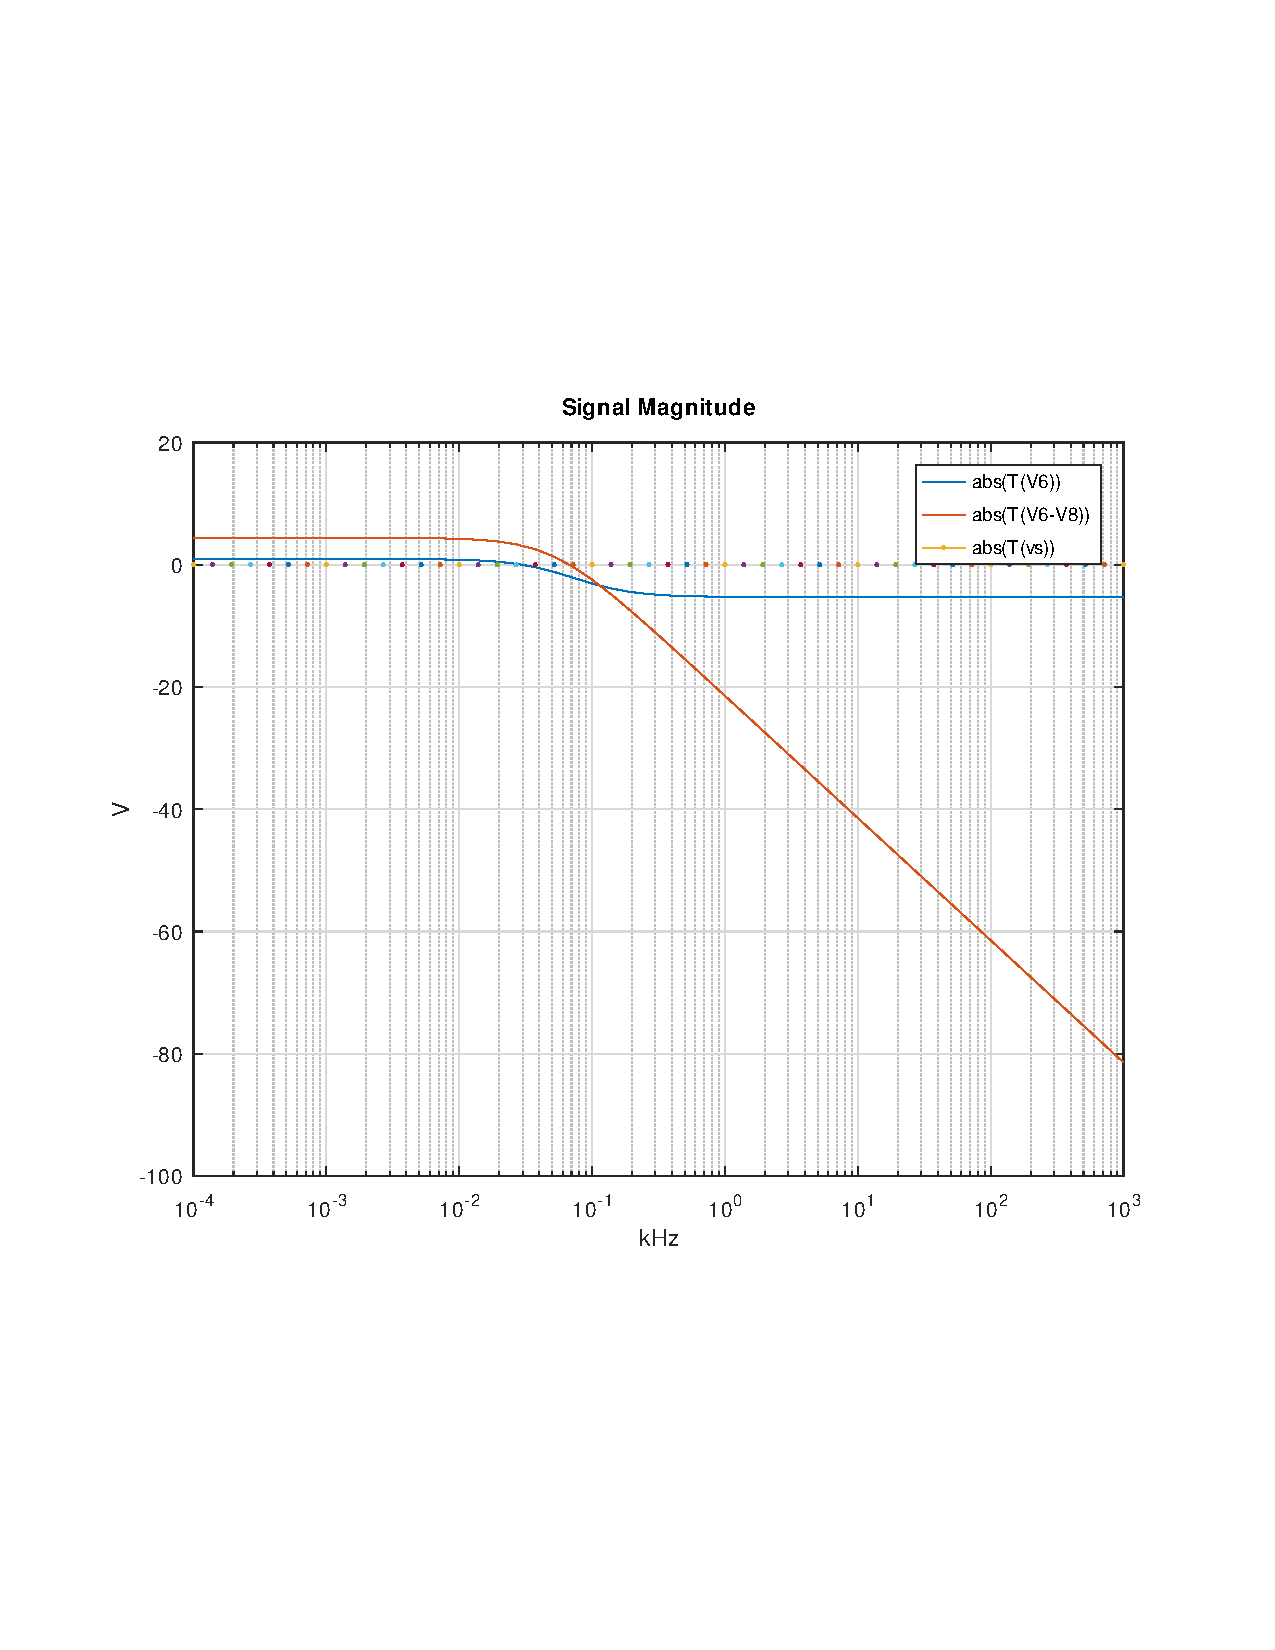
\includegraphics[width=0.6\linewidth]{../mat/TransAbs.pdf}
\caption{Forced solution $t > 0$s}
\label{fig:TForcedP}
\end{figure}

\begin{figure}[h!] \centering
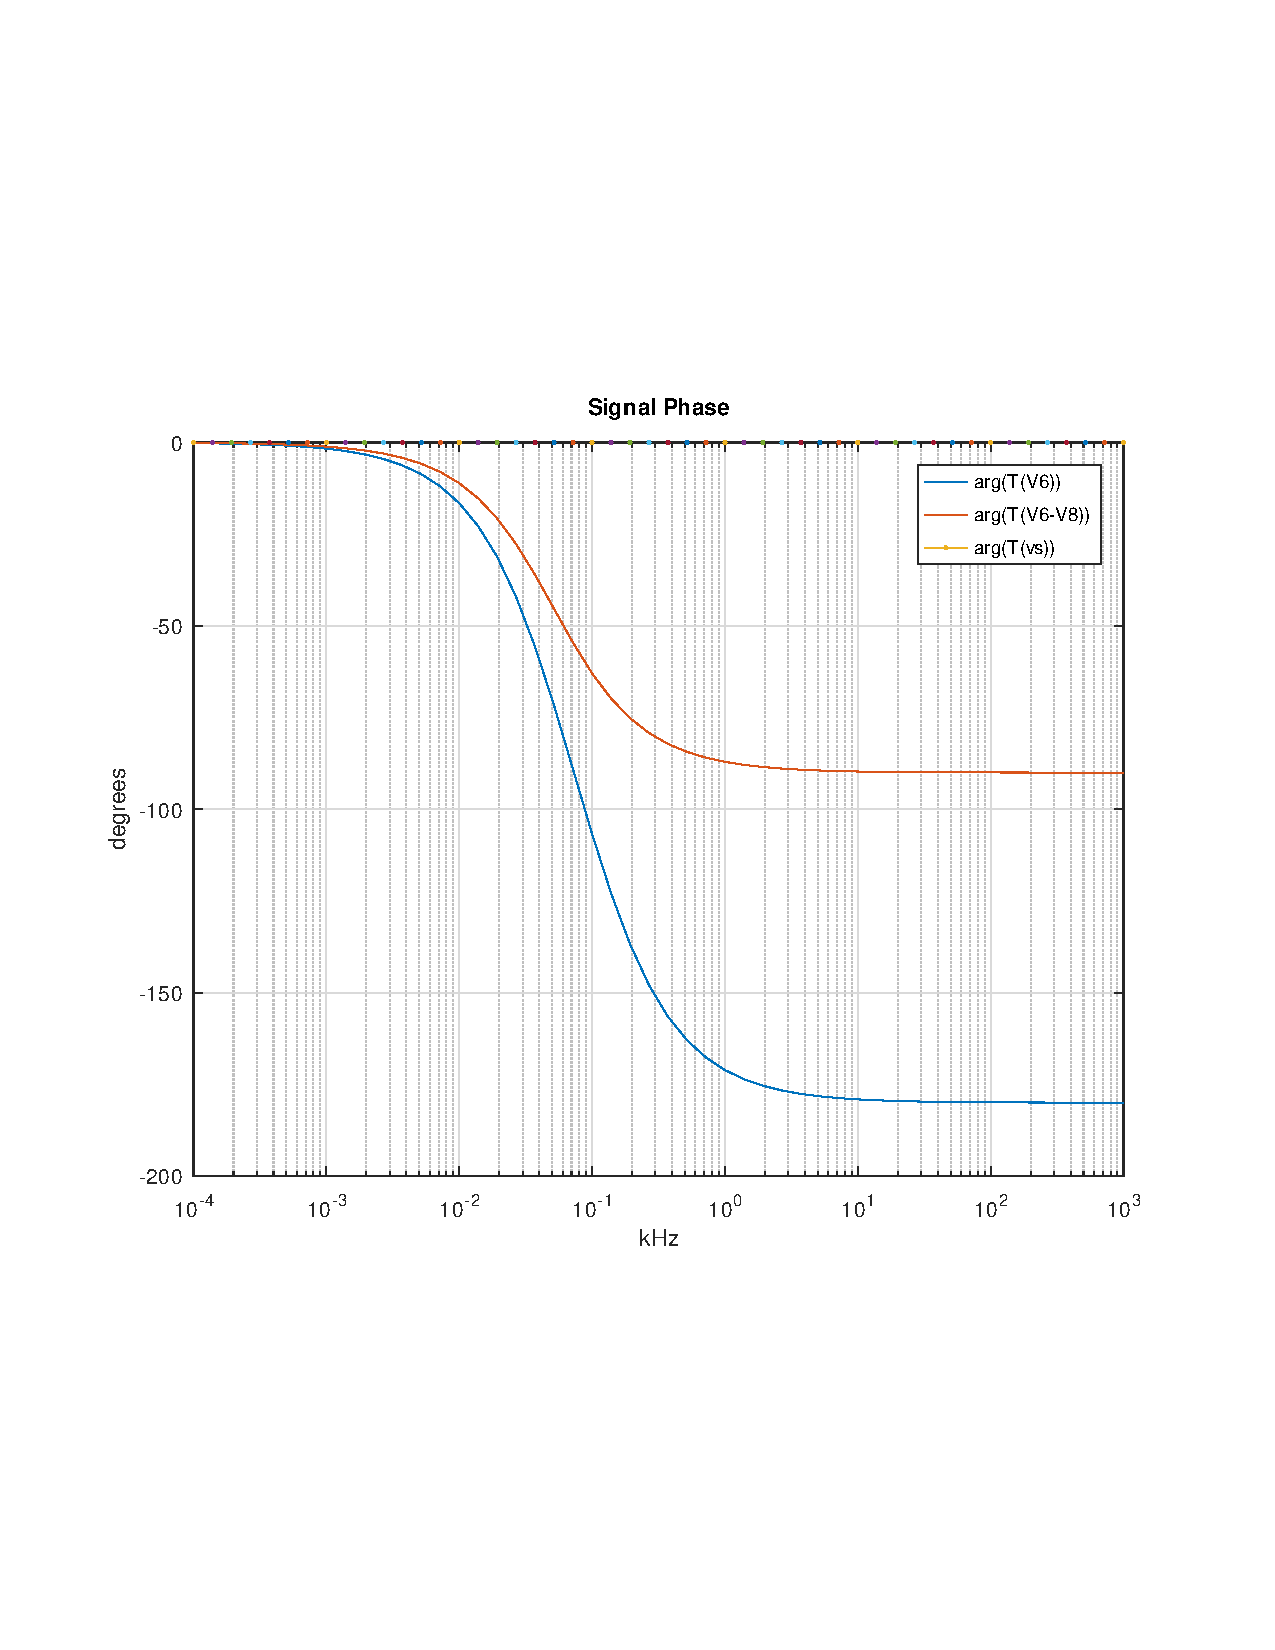
\includegraphics[width=0.6\linewidth]{../mat/TransPha.pdf}
\caption{Forced solution $t > 0$s}
\label{fig:TForcedP}
\end{figure}

\newpage

